\documentclass[12pt]{report}
\usepackage{graphicx} % Required for inserting images
\linespread{1.2}

\usepackage[dvipsnames]{xcolor}
\usepackage{tikz}
\usepackage[breakable]{tcolorbox}
\appto{\bibsetup}{\raggedright}

\tikzstyle{mybox} = [draw=PineGreen, fill=PineGreen!5, ultra thick, rectangle, rounded corners, inner sep=10pt, inner ysep=15pt, text width=0.90\textwidth, align=left] 
\tikzstyle{boxtitle} = [fill=PineGreen, text=white, ultra thick, rectangle, rounded corners, inner sep=10pt, inner ysep=8pt, text width=0.90\textwidth]

\newcommand{\BoxDef}[2]{%
\vspace*{10px}
\noindent

\begin{center}
\begin{tikzpicture}
    \node[mybox](box){\rule{0pt}{30pt}\ignorespaces#2\unskip};
    \node[boxtitle, anchor=north west] at (box.north west) {\textbf{#1}};
\end{tikzpicture}
\end{center}
}

\newcommand{\ceil}[1]{\left\lceil#1\right\rceil}

\newcommand{\floor}[1]{\left\lfloor#1\right\rfloor}

\usepackage[]{hyperref}
\usepackage{amsfonts}
\usepackage{amsmath}
\usepackage{amssymb}
\usepackage{dsfont}
\usepackage{bm}
\usepackage[top=2.5cm, bottom=2.5cm, left=3cm, right=3cm, centering]{geometry}
\usepackage{algorithm}
\usepackage{algpseudocode}
\usepackage{tabularx}
\usepackage{tabularray}
\usepackage{svg}
\usepackage{enumitem}

\begin{document}

\begin{titlepage}
\hrule
\vspace{15pt}
\begin{center}
    \Huge{\textbf{\Huge \textbf{Information Retrieval 24-25}} \\ Notes}\\
\end{center}
\vspace{15pt}
\hrule
\vfill
\hrule
\begin{center}
    \Large University of Pisa \\ M.Sc. in Computer Science
\end{center}
\end{titlepage}

\tableofcontents

\chapter{Introduction}

Information retrieval is the process of finding relevant material of unstructured nature from large collections. The ``material'' is usually documents, web pages, or multimedia content. Originally, information retrieval was something only a few professionals interacted with. Nowadays, hundreds of millions of people engage with information retrieval systems when they, for example, use a web search engine or search through their email.

The two key aspects considered when evaluating the quality of an IR system are \textbf{effectiveness} and \textbf{efficiency}. The first refers to the capability of the system to produce a satisfactory result; the second refers to how quickly it does so. To guarantee a certain level of quality, some operations are done offline, such as document indexing, feature processing (e.g., term frequency, metadata), training of a learn-to-rank model to produce the order in which documents will be shown to the user, and so on. Still, many operations must be done on-line, such as query expansion and processing, index and feature lookup, and usage of the ranking funcion. If we consider the example of a search engine (SE), we are used to getting back a response in a very short amount of time, despite the fact that in order to find the collection of documents presented to us, a lot of different operations must have been performed (i.e., the system must be efficient). Additionally, we also expect that those documents are the most relevant ones found in the collection, and that they are presented in the order of relevancy (the system must be effective). If those two ideas do not hold, we're unlikely to actually use the system for an extended amount of time.

The following chapters will go in detail about the different components of IR systems, and each will focus on how effectiveness and efficiency can be guaranteed. The key aspects that will be considered are:
\begin{itemize}
    \item \textbf{Language properties:} how does language influence retrieval? What does it mean to retrieve a piece of text? How are documents scored and presented?
    \item \textbf{Auxiliary data structures:} e.g., inverted indexes;
    \item \textbf{Query processing:} how are queries expanded from the form provided by the user into one which can be ``read'' by the system?
    \item \textbf{Data storage and compression:} how can data be compressed efficiently?
    \item \textbf{Learning-to-rank models:} how is machine learning used in an IR system to produce a ranking (based on available ranked data)?
    \item \textbf{Neural IR:} how can Deep Learning and specifically Large Language Models be used in IR?
\end{itemize}
\chapter{Evaluation}

To evaluate the quality of an IR system, say a SE, we may ask questions such as: how fast does it index a collection, how fast does it search (efficiency)? Or, does it recommend good related pages/products to buy to the user (effectiveness)? However, these questions alone do not provide any objective information about the intrinsic quality of the SE. We could say that a SE is ``good'' if it makes its users happy; but to measure this happiness, we can use different definitions: for example, how many times a search result is clicked, how long users stay on the same webpage, how often they return to use the SE. Since happiness by itself is impossible to measure, a commonly used proxy is \textbf{relevance} of search results.

\section{Relevance}

In order to measure relevance, three elements are needed:
\begin{itemize}
    \item A benchmark document collection;
    \item A benchmark suite of queries;
    \item An assessment of either \textbf{relevant} or \textbf{non-relevant} for each query and document.
\end{itemize}
To construct the benchmark, we would have to analyze each possible pair of query and document and assign a relevance to it. Relevance assessment can be binary (relevant/not relevant), or multi-valued (0, 1, 2, 3 ...) for more nuance. Obviously, since assigning a relevance value to each query-document pair in a collection is way too expensive, a subset of the documents is used instead.

Assigning relevance must be done externally by humans. Some companies use crowdsourcing platforms (e.g., Amazon Mechanical Turk) to present pairs to low cost, not highly qualified workers. This solution is cheap, but the outcome may not be as good as one produced by professionals. 

But how are the queries defined? They must be relevant and suitable to the documents in the collection, and must be representative of user needs (i.e., they should resemble a normal query done by a person). One way to find them is to sample directly from existing query logs of the SE, if available. For classical, non-Web IR systems, these query logs may be nearly empty, as the query rate tends to be slow. In this case, experts may handcraft ``user needs'' and associated queries. Among popular public test collections is \textbf{TREC} (\textbf{Text REtrieval Conference}), where focus areas are called \textbf{tracks}; each track has a motivating use case, usually an abstraction of a user task. In practice, TREC consists of:
\begin{itemize}
    \item A set of documents;
    \item A set of information needs (called \textbf{topics});
    \item Relevance judgements that indicate which documents should be retrieved by which topics.
\end{itemize}
The result of a retrieval system executing a task on a test collection is called \textbf{run}. The technique first used to select the sample of documents to present to a human judge is \textbf{pooling}: the top results for a set of runs are combined to form a pool and only those documents are judged. Since this method automatically assumes that all unpooled documents are not relevant (so they remain unjudged), alternative methods have been investigated by TREC tracks to obtain judgements that support fair evaluation.

Note that TREC does not contain any query, and only generic user needs. Participants are free to define (manually or automatically) actual queries for their specific IR system.

\subsection{Measures}

\subsubsection{Evaluation of Unranked Retrieval Sets}

\textbf{Precision} and \textbf{recall} are binary assessments commonly used to evaluate the effectiveness of an IR system. They are defined on the basis of a set of counts, described by the table below.
\begin{table}[ht]
    \centering
    \begin{tabular}{|c|c|c|}
         \hline
         & Retrieved & Not retrieved \\
        \hline
        Relevant & TP & FN \\
        \hline
        Non-relevant & FP & TN \\
        \hline
    \end{tabular}
\end{table} \\
The two measures are then defined as:
\begin{itemize}
    \item \textbf{Precision:} fraction of retrieved documents that are relevant.
    \begin{equation*}
            \textit{Precision} = \frac{TP}{TP + FP}
    \end{equation*}
    
    \item \textbf{Recall:} fraction of relevant documents that are retrieved.
    \begin{equation*}
        \textit{Recall} = \frac{TP}{TP + FN}
    \end{equation*}
\end{itemize}
The \textbf{F-Measure} (or \textbf{F-Score}) is another metric which condenses both precision and recall; it's calculated as the harmonic mean of the two:
\begin{equation*}
    F = \frac{1}{0.5 \textit{Prec.} + 0.5 \textit{Rec.}} = 2 \frac{\textit{Prec.} \cdot \textit{Rec.}}{\textit{Prec.} + \textit{Rec.}}
\end{equation*}
The harmonic mean is alway less or equal than the arithmetic/geometric mean: if the two values are very different, the harmonic mean is closer to their minimum. A weighted variant also exists; let $\alpha$ be the weight assigned to precision and $\beta$ the weight assigned to recall, such that $\alpha = 1/(1+\beta^2)$, \textbf{weighted F-Measure} is calculated as:
\begin{equation*}
    F_{\beta} = (\beta^2 + 1)\frac{\textit{Prec.} \cdot \textit{Rec.}}{\beta^2 \textit{Prec.} + \textit{Rec.}}
\end{equation*}

\subsubsection{Evaluation of Ranked Retrieval Results}

Precision, recall, and F-score are set-based methods, meaning that they are computed using an unordered set of documents. They can be extended to evaluate the ranked retrieval results returned by search engines. Some of these measures are \textbf{Mean Average Precision} (\textbf{MAP}), \textbf{Precision@K} (\textbf{P@K}), \textbf{Mean Reciprocal Rank} (\textbf{MRR}) for binary relevance, and \textbf{Normalized Discounted Cumulative Gain} (\textbf{NDCG}) for multiple levels of relevance.

\paragraph{Mean Average Precision}

Consider a set of documents in a run, classified as relevant or not relevant by the SE. Consider the indexes $K_1, \dots, K_R$ at which recall increases (i.e., the indexes of the actually relevant documents in that run). Precision is calculated at each $K_i$, considering only the documents with lower indexes, and the average across all $K_i$ is calculated at the end. MAP is then calculated as the mean of the averages across multiple queries/rankings, as a measure of the whole system given that benchmark.

MAP is a macro-averaging measure; each query counts equally, even if only few documents are relevant for certain queries and many are relevant for other queries.

\paragraph{Precision@K}

MAP takes into account all documents returned by the query. However, especially in Web searches, the number of retrieved documents may be unknown or very high; what truly matters is how any good results are found in the first few pages. To calculate Precision@K, we set a rank threshold $K$, we compute the number of relevant documents among the top $K$ ranking ones, and calculate P@K as:
\begin{equation*}
    P@K = \frac{\sum \textit{relevant and retrieved documents in top-K}}{K}
\end{equation*}
i.e., it is the fraction of relevant documents across the top-K retrieved ones (which are assumed to be relevant by the system). In a similar fashion, we also calculate \textbf{Recall@K} as the fraction of relevant documents that are found among the top-K:
\begin{equation*}
    R@K = \frac{\sum \textit{relevant and retrieved documents in top-K}}{\textit{\# of relevant documents}}
\end{equation*}

P@K by itself does not average very well over a set of queries, since the number of relevant documents for a query affects the result. Anyway, it (along with \textbf{MAP@K}) are largely used for Web searches and recommender systems.

\paragraph{Mean Reciprocal Rank}

Suppose there is only a single relevant document for a given query. A way to approximate the rank of the correct answer could be to consider the search duration for the user: if its ranking is low, he/she takes a long time to find the answer; if it is ranked high, he/she finds it quickly.

Consider the rank position $\textit{rank}_i$ of the first relevant document returned by a query $q_i \in Q$. The \textbf{Reciprocal Rank} is calculated as:
\begin{equation*}
    \textit{RR} = \frac{1}{\textit{rank}_i}
\end{equation*}
MRR is the mean of the RRs across multiple queries.

\subsubsection{Evaluation of Non-Binary Relevance}

A popular measure used to evaluate web searches with non-binary relevance is \textbf{cumulative gain}, and in particular \textbf{Normalized Discounted Cumulative Gain} (\textbf{NDCG}). The idea is that the lower the rank of a relevant document is, the less it is useful for the user, since it is less likely to be visited.

Discounted Cumulative Gain uses graded relevance (or \textbf{gain}) as a measure of usefulness; it is accumulated starting at the top of the ranking and may also be discounted (= reduced) at lower ranks. The typical discount is $\frac{1}{\log(\textit{rank})}$. Let $r_i$ be the relevancy of the document; then, DCG is calculated as:
\begin{gather*}
    \textit{DCG} = r_1 + \frac{r_2}{\log_2 2} + \frac{r_3}{\log_2 3} + \dots + \frac{r_n}{\log_2 n} = \\
    = r_1 + \sum_{i=2}^n \frac{r_i}{\log_2 i}
\end{gather*}
This case uses base 2 for the logarithm, but any other base can be used as well. As for the other measures, it can be calculated only for the $p$ top ranking documents instead of the whole set of retrieved ones.

An alternative formulation makes it so that high relevance judgements become much more important:
\begin{equation*}
    \textit{DCG} = \sum_{i=1}^n \frac{2^{r_i} - 1}{\log_2(1+i)}
\end{equation*}
This variant is used by some web search companies.

NDCG is the normalized version of DCG, and is calculated as the ratio between the DGC of a response and the ideal DGC of a perfect ranking; the perfect ranking would be one that first returns all the docuents with the highest relevance level, then the next highest relevance level, and so on.
\begin{equation*}
    \textit{NDCG} = \frac{DCG}{\textit{Ideal} \ DGC}
\end{equation*}
NDCG takes values between 0 and 1.
\chapter{Efficient Algorithms for Modern CPUs}

Modern IR systems must manage billions of documents and queries, so we need efficient algorithms that can handle such amounts of data, as well as scale across global infrastructures. Efficiency does not only mean a better user experience, but also a reduction in costs, both for computing and cooling systems. Additionally, efficient systems consume less energy, and therefore are more environmentally sustainable.

Computers use several layers of cache on their chips to speed up RAM and disk access time. When an instruction or a block of data must be read, it is also stored accordingly into the cache(s), since they are faster to access. The smaller the cache, the faster the access time. Ideally, programs should take in consideration how cache layers are used and exploit temporal and spatial locality.
\begin{itemize}
    \item \textbf{Temporal locality} states that when a block of data has been accessed, it is likely to be accessed again very soon. Cache replacement policies such as LRU make sure to keep the data that is most likely to be needed.
    \item \textbf{Spatial locality} states that when a block of data has been accessed, it is likely that nearby memory locations will also be accessed in the near future.
    
    Normally, when a location is accessed, a larger chunk of memory is read (a cache line of 64 bytes). \textbf{Hardware prefetchers} can observe the behaviour of a program and prefetch data if repetitive patterns of cache misses appear.
\end{itemize}

\section{Parallelism}

Another interesting thing to consider is \textbf{parallelism}. Parallelism can speed up a CPU through:
\begin{itemize}
    \item \textbf{Pipelining}, which overlaps the execution of multiple instructions so that different parts of the CPU are kept busy at the same time;
    \item \textbf{Superscalar processors}, which have multiple execution units that process independent operations simultaneously;
    \item \textbf{SIMD}, which are a special kind of instructions executing the same operation on more data at the same time.
\end{itemize}

\paragraph{Pipelining}
When an instruction is executed, it actually goes through multiple stages on the CPU. The most simple pipelining is a 5-stage one: fetch, decode, execute, load/store, write. The time needed to move an instruction from one stage to the other defines the \textbf{clock time}, so it is chosen to accomodate the longest possible operation (usually memory access). 

Modern high-performance CPUs have multiple pipeline stages, usually 10-20, but may be more. This means that the latency to execute something simple like an \texttt{add} operation may need up to 20 or more cycles. \textbf{Latency} is the total time that an operation passes in the pipeline, while \textbf{throughput} of a CPU is the number of instructions that are completed and exit the pipeline per unit of time.

\textbf{Pipeline hazards} are situations where the next instruction cannot go forward in the pipeline in the next clock cycle. This can happen because of:
\begin{itemize}
    \item \textbf{Structural hazards}, when one or more instructions must wait because another one further in the pipeline is using a component. These hazards are unavoidable.
    \item \textbf{Data hazards}, when an instruction must wait for an operand to be computed from a previous step. They can be avoided by restructuring computation;
    \item \textbf{Control hazards}, when the CPU cannot tell which branch in an \texttt{if-else} statement it must choose. Normally, it will choose randomly and keep loading instructions into the pipeline, and, if the choice turns out to be wrong, the pipeline will be flushed to accomodate the correct branch (thus wasting some cycles).
\end{itemize}
Regarding the last type, thankfully CPUs have \textbf{branch predictors} capable of guessing which branch is the more likely to be picked by observing past behaviour. The branch predictor is capable of noticing particular patterns, such as a condition holding true/false for several loop iterations, or a condition alternating between true/false between successive instructions.

\paragraph{Superscalar Processing}
In superscalar processing, multiple instructions are dispatched to do different execution units on the core (each core has several specialized ALUs). This type of parallelism is also called \textbf{instruction-level parallelism}.

\paragraph{Single Instruction, Multiple Data}
SIMD instructions operate n special registers that hold 128, 256, or even 512 bits. Data in registers is divided into blocks of 8, 16, 32, or 64 bits.

SIMD instructions can be used in two ways: either through \textbf{auto-vectorization}, meaning that the compiler automatically converts scalar operations into SIMD ones, or they are explicitly used by the programmer in the code. In the latter case, there is an higher level of control over which operations are optimized (since the automatic conversion done by the compiler can only optimize simpler instructions), but obviously requires detailed hardware knowledge.
\chapter{Natural Language}

Natural language is the language used by humans to communicate with each other. Languages are defined on the basis of thousands of words, a complex syntax, and a mostly compositional semantic. Language is also often ambiguous; the same word may have different meanings depending on the context of the sentence, or the same sentence may be interpreted in different ways.

\textbf{Natural Language Understanding} has the aim of building machines capable of receiving and giving information using natural language, like a human would. Natural language processing is said to be an ``AI-complete'' problem, meaning that it is a problem only solvable using AI, and that if we were to find a solution, then we'd have a solution for any other problem. In practice, natural language processing is used in many applications, such as chatbots, search engines, machine translation, and personal assistants (such as Alexa by Amazon, or Google Home by Google). It can be used with different data types: tabular data (to construct and interpret search queries), graphs (to represent the content of each node and link, for example in a social media graph), and images/video data (to describe the content of the image/video and to retrieve or generate similar images/videos).

Information Retrieval is strictly connected and overlapping with the fields of Natural Language Processing and Machine Learning:
\begin{itemize}
    \item NLP methods are often built on top of IR or ML methods;
    \item ML uses IR measures to define the goals of the learned models, and assumes language can be manipulated via NLP.
\end{itemize}

\section{NLP Pipelining}

A \textbf{processing pipeline} is a sequence of preprocessing steps aimed at transforming the raw text input into a format that can be effectively used as input to the chosen machine learning model(s). Some of the key steps in the pipeline are:
\begin{itemize}
    \item \textbf{Tokenization}: it identifies the words (tokens) in the text. Popular libraries provide ``language aware'' tokenization, i.e., it isolates tokens differently depending on the language or context of the text. After this step, a \textbf{vocabulary} of the terms used can be constructed.
    \item \textbf{Sentence splitting}: it isolates whole sentences from the text, so that they can be analyzed individually. This is not always an easy task, as punctuation marks can often be used for uses other than sentence separation (e.g., in acronyms, numbers, initials, etc.).
    \item \textbf{Stemming and lemmatization}: both aim at reducing words to their roots; stemming does it by applying a set of language-dependent transformation rules to find the stem of a word, while lemmatization actually tries to find the root of the word in the vocabulary. The difference between the two can be shown with an example: the word ``cars'' is both stemmed and lemmatized to ``car''; the word ``was'' may be stemmed to ``wa'', but lemmatized to ``be''.
\end{itemize}
Raw text can be transformed in different formats depending on the task to be solved. Common models are bag-of-words and n-grams.

\textbf{Bag-of-words} represents a text as the list of unique words appearing in it. It loses any information about word frequency and order, requiring external data structures to store this information; on the other hand, it is easy to implement and calculate. The set of all distinct extracted words can be called \textit{dictionary}, \textit{vocabulary}, or \textbf{feature set/space}, since each word becomes a feature of the new representation.

\textbf{N-grams} features are sequences of $n$ words which capture word order. They do not correspond to a specific token in the text, and are instead obtained as a combination of them. For example, in the text:
\begin{center}
    \textit{``the quick brown fox jumps over the lazy dog''}
\end{center}
we can find 2-grams such as:
\begin{center}
    \textit{'the quick'', 'quick brown', 'brown fox', ... , 'the lazy', 'lazy dog'}
\end{center}
Different libraries have specific formats to identify n-grams.

\section{Zipf's Law}

Zipf's Law is an empirical law used to model the frequency of words in a text. It is based in the observation that the most common word in a text is usually twice as frequent as the second most common one, three times as frequent as the third most common, and so on. Specifically, the law states that the frequency of a word is proportional to the inverse of the rank:
\begin{equation*}
    \textit{frequency} = \frac{1}{(\textit{rank} + b)^a}
\end{equation*}
where $a \approx 1$, $b \approx 2.7$.

\begin{figure}[ht]
    \centering
    \includesvg[width=0.75\textwidth]{img/zipf.svg}
    \caption{Plots showing the frequency of words (in the English language) according to Zipf's Law.}
    \label{fig:zipf}
\end{figure}

The \textbf{principle of least effort} is a theory that states that animals, people, and even well-designed machines naturally choose the path of least effort, meaning the one that requires the least amount of work to reach a goal. In the case of human communication, both speaker and listener in a conversation will abide by this principle. The speaker tends to use a small vocabulary of common words, while the listener tends to prefer longer, rarer words. Zipf's Law can be seen as the result to the compromise between the two.

\textbf{Stopwords} are the most common words in a language. In the English lanaguage, stopwords include ``the'', ``a'', ``to''. They can be removed from the text without losing too much information. Different libraries and tools provide their own list of stopwords depending on the application; for example, MySQL specifies words such as ``appreciate'' or ``unfortunately'', since it's used for sentiment analysis.

When it comes to rare words, it is not necessarily true that uncommon words are the most informative or useful. If a word is so rare that it appears very few times in very few documents, it may actually be of little help for future retrieval: it could be a typo, or a sort of artificial identifier associated to the document (e.g., a slug in a url). Removing these rare words can help make it faster to process indexed data, and requires less space.

\section{Vector Space Model}

Words can be represented as $|F|$-dimensional vectors obtained through \textbf{one-hot encoding}, where $F$ is the set of distinct features (words, n-grams, etc.) in the collection. The relevance of a feature $f$ in the document $d$ is indicated as $w_{f,d}$.

A document can then be represented as the weighted sum of all the vectors of its features:
\begin{equation*}
    v(d) = \sum_{f \in d} w_{f,d} v(f)
\end{equation*} 
These vector representations are usually sparse (most of their terms are equal to 0). Weights can be assigned in different ways. Common methods are binary weights (bag-of-words), term frequency (tf), and tf-idf.

To find matches between a query and a document, we can compare the terms appearing in both: using a simple boolean operator (AND/OR), we can check wheter a certain document contains only/all the terms in the query and return them to the user. This is a very simple methodology, but it does not produce a ranking and does not take into account the frequency of words.

In \textbf{ranked retrieval}, the system reorders the (top $k$) documents in the collection for a given query. Instead of defining binary queries with a specific language, natural language is used instead. To rank documents, we need some way to assign a \textbf{score} to each document given a query that measures how well they match.

A possible scoring is given by \textbf{Jaccard's coefficient}:
\begin{equation*}
    \textit{jaccard}(A,B) = \frac{|A \cap B|}{|A \cup B|}
\end{equation*}
where $A$ and $B$ are sets (in our case, the query and the document). This coefficient is always a value between 0 and 1, where 0 means no overlap and 1 means perfect overlap. While a better alternative than basic binary scoring, it is based on the assumpion that its operators are sets, so it does not consider term frequency to calculate the score. The more frequent is the term in the document, the higher the score; the rarer the term in a collection, the more informative it is (with the exceptions mentioned above).

\subsection{TF-IDF Scoring}

We introduce two data structures to then define more sophisticated scoring measures: the incidence matrix and the count matrix. \\
The \textbf{incidence matrix} is used to represent the presence of absence of terms in documents. Each row corresponds to a word, and each column corresponds to a document.
\begin{table}[!ht]
    \centering
    \begin{tabular}{c|cccc}
        & $d_1$ & $d_2$ & $d_3$ & $d_4$ \\
        \hline
        $w_1$ & 1 & 0 & 1 & 0 \\
        $w_2$ & 0 & 1 & 0 & 1 \\
        $w_3$ & 1 & 1 & 0 & 0 \\
        $w_4$ & 0 & 0 & 1 & 1 \\
    \end{tabular}
    \caption{Example of an incidence matrix.}
    \label{tab:incidence-matrix}
\end{table} \\
The \textbf{count matrix} keeps track of the number of occurrences of a term in a document, so each column of the matrix is a count vector, and each count vector is a multiset.
\begin{table}[!ht]
    \centering
    \begin{tabular}{c|cccc}
        & $d_1$ & $d_2$ & $d_3$ & $d_4$ \\
        \hline
        $w_1$ & 32 & 0 & 5 & 0 \\
        $w_2$ & 0 & 15 & 0 & 13 \\
        $w_3$ & 2 & 1 & 0 & 0 \\
        $w_4$ & 0 & 0 & 10 & 2 \\
    \end{tabular}
    \caption{Example of a count matrix.}
    \label{tab:count-matrix}
\end{table} \\
Note that this representation still does not consider the order in which words appear in the documents.

The \textbf{term frequency} $\textit{tf}_{t,d}$ of a term $t$ in a document $d$ is simply the number of times $t$ appears in $d$. Raw term frequency cannot be used as is, however, since relevancy is not linearly proportional to it. A document with 10 occurrences of a term is more relevant than a document with only 1 occurrence, but it is not 10 times more relevant. \textbf{Log-frequency weight} is a common way to normalize term frequency:
\begin{equation*}
    w_{t,d} = \begin{cases}
        1 + \log_{10}(\textit{tf}_{t,d}) & \textit{tf}_{t,d} > 0 \\
        0 & \text{otherwise}
    \end{cases}
\end{equation*} 
The score of a document-query pair is then calculated by summing the weights of all the terms appearing in both:
\begin{equation*}
    \textit{score}(q,d) = \sum_{t \in q \cap d} w_{t,d}
\end{equation*}
The score is always 0 if none of the terms of the query appear in the document.

However, we previously mentioned that informativeness also depends on how frequent the word is in the entire collection. If a term is globally rare, documents containing that word will be more relevant for queries asking for it. To capture this aspect, \textbf{document frequency} $\textit{df}_t$ is used: it is defined as the number of documents containing term $t$. Since $\textit{df}_t$ measures the inverse of the informativeness of a word, \textbf{inverse document frequency} ($\textit{idf}_t$) is used instead:
\begin{equation*}
    \textit{idf}_t = \log_{10} \left(\frac{N}{\textit{df}_t}\right)
\end{equation*}
where $N$ is the number of documents in the collection. The logaritm is used for the same reason as for term frequency. Inverse document frequency by itself cannot rank documents in one-term queries, since $\textit{idf}$ is always either 0 if the document does not contain the term, or a positive value if it does (obtained by the formula above). For multi-term queries, scoring is given by:
\begin{equation*}
    \textit{score}(q,d) = \sum_{t \in q \cap d} \textit{idf}_t
\end{equation*}
In this formula, the role of the document is to filter out the terms which contribute to its own ranking.

These two measures are combined into what's known as \textbf{tf-idf weighting}, which is the product between them:
\begin{equation*}
    \textit{tf-idf}_{t,d} = w_{t,d} \cdot \textit{idf}_t
\end{equation*}
This is the most common weighting scheme in Information Retrieval. Scoring of a document-query pair is calculated as:
\begin{equation*}
    \textit{score}(q,d) = \sum_{t \in q \cap d} \textit{tf-idf}_{t,d}
\end{equation*}
There are many variants which differ in the way the components are weighted, or the way single terms in the query are weighted as well. \\
A frequently used variant is \textbf{Best Match 25} (\textbf{BM25}), which calculates the score as:
\begin{gather*}
    \textit{score}(q,d) = \sum_{t \in q \cap d} \textit{idf}_t \cdot \frac{\textit{tf}_{t,d} \cdot (k_1 + 1)}{\textit{tf}_{t,d} + k_1 \cdot (1 - b + b \cdot \frac{|D|}{\textit{avgdl}})} \\
    \textit{idf}_t = \ln \left( \frac{N - \textit{df}_t + 0.5}{\textit{df}_t + 0.5} + 1 \right)
\end{gather*}
where $|D|$ is the length of the document (how many words it contains), \textit{avgdl} is the average length of the documents in the collection, and $b, k_1$ are hyperparameters; $b \in [0,1]$ and $k_1 \in [1.2,2.0]$.

\subsection{Vector Space Similarity Scoring}

Since \textit{tf-idf} can be calculated for each term-document pair, we can construct an additional data structure, called \textbf{weight matrix}, which stores all these values. Each document (which is a column in the matrix) can be then thought of as a vector representing a point in $\mathbb{R}^{|F|}$.

The scoring introduced above, however, still presents a problem. Ideally, we want to consider not only the relevancy of single words, but also how relevant a document is in the entire collection. If a document has many rare terms, it should rank higher than another document which has less rare terms. To solve this issue, we can rank  documents according to how similar/distant they are from the query (which can be represented as a $|F|$-dimensional vector as well).

A first similarity measure is \textbf{Euclidean distance}. It is simple to calculate, and does return a value that is greater the more distant the two vectors are in the space considered. However, Euclidean distance can end up being way too high for vectors of different lenghts (i.e., unnormalized), even if they have the same orientation: for example, consider a document $d$ and append it to itself, obtaining $d'$. Even though the two documents have the same content (and will have the same direction in the vector space), their magnitude is different, with $d'$'s being exacly double that of $d$. The key idea is then to rank documents depending on the angle forming between them.

Ranking documents in decreasing order of the angle between query and document is equivalent to ranking them in increasing order of the cosine of the angle. This measure is called \textbf{cosine similarity}:
\begin{gather*}
    \cos(\theta) = \frac{q \cdot d}{\|q\| \cdot \|d\|} = \frac{\sum_{i=1}^{|F|} q_i d_i}{\sqrt{\sum_{i=1}^{|F|} q_i^2} \cdot \sqrt{\sum_{i=1}^{|F|} d_i^2}}
\end{gather*}
Note that here vectors are length-normalized by dividing each for its L2 norm. In the previous example, $d$ and $d'$ would end up having the same lenght after being normalized, so their cosine similarity would be 1 (the maximum possible value).

Different search engines can use different weighting and different normalizations to calculate \textit{tf-idf} and vector similarity. In the \textbf{SMART} notation, each method is associated to a different letter (e.g., n for natural/no weighting, l for logarithm, b for boolean, etc.), and the combination used by the engine is specified by a string of six letters: \textit{ddd.qqq}. Different weightings can be used for queries and documents. A standard scheme is \textbf{\textit{lnc.ltc}}: logarithmic \textit{tf}, no \textit{idf}, cosine similarity normalization for documents, and logarithmic \textit{tf} \textit{idf}, and cosine similarity normalization for queries.
\chapter{Indexing}

When a user query is submitted to an IR system, the terms in the query must be compared to those contained in the documents in the collection in order to retrieve the relevant ones. If these systems were to use the vector/matrix representation of queries and documents as they are, the complexity of the retrieval would be too high to provide a reasonable response time: we'd need to compute the similarity (i.e., product) between the query vector and all the document vectors in the collection, which are many and with a high number of dimensions. However, these representations tend to be very sparse, meaning that a lot of information could be summarized in a more compact form.

\textbf{Inverted indexes} are the most effective data structures used in IR systems for efficient query processing. They consist of a collection of lists (called \textbf{posting lists}), each corresponding to a term in the collection and containing information about the documents in which the term appears in. Each term in the index is also accompanied by its document frequency and its collection frequency; each document ID in the posting list is accompanied by the term frequency in that document. Document IDs are kept sorted in increasing order.

Inverted indexes are often stored in main memory to reduce access time; since they can be very big (the dictionary usually contains a huge number of distinct terms, and the collection holds a huge number of documents), lossless compression algorithms are used to reduce their size.
\clearpage
\begin{figure}[!h]
    \centering
    \includesvg[width=0.75\textwidth]{img/inverted_index.svg}
    \caption{Example of inverted index.}
    \label{fig:inverted-index}
\end{figure}

\section{Query Processing}

This section will illustrate the fundamental query processing strategies for Boolean retrieval (when an exact answer is required), and ranked retrieval (when a ranked list of scored documents is required). We will assume that the query has already been pre-processed. The two classical query processing strategy categories are \textbf{term-at-a-time} (\textbf{TAAT}), and \textbf{document-at-a-time} (\textbf{DAAT}).

\paragraph{TAAT}
In TAAT, posting lists are read one query term at a time, and accumulators are used to keep track of the documents that satisfy the query; these accumulators may be simple counters or sum up the document score. Accumulators are normally stored in a direct access table or hash table: the first data structure uses the document ID as the key to access the accumulator, while the second uses a hash key calculated from the document ID. If a query is in conjunctive (AND) mode, only the IDs with accumulators equal to the number of query terms are returned; if it is in disjunctive (OR) mode, all the IDs with non-zero accumulators are returned. These approaches are very simple to implement but tend to produce a lot of cache misses because of the large number of accumulators needed. Also, there is no way to skip document IDs for selective queries.

\paragraph{DAAT}
In DAAT, the posting lists of all the query terms are scanned in parallel, calculating the document score when it is seen in one or more posting lists. Depending on the mode of the query, a different strategy is used:
\begin{itemize}
    \item For OR queries, the union of all the posting lists must be computed. The lists are scanned in parallel and merged with the same approach used in the merge phase of a K-way Merge Sort.
    \item For AND queries, the intersection of all posting lists must be computed. Similarly to before, the lists are scanned in parallel, adding an ID to the result only if all the pointers are pointing to that same ID, otherwise advancing the pointer(s) with the lowest ID without adding anything to the result.
\end{itemize}

\subsection{Efficient Document ID Searching}

The main operations on posting lists are:
\begin{itemize}[itemsep=0pt]
    \item[-] \texttt{first}(): places the pointer to the first docID
    \item[-] \texttt{docID}(): returns the current docID
    \item[-] \texttt{position}(): returns the position of the pointer
    \item[-] \texttt{next}(): moves the pointer to the next docID
    \item[-] \texttt{nextGEQ}($d$): moves the pointer to the next docID that is greater or equal than $d$
\end{itemize}
This last operation allows us to skip some document IDs, without having to scan all the posting list; this is useful when the query to be processed is in AND mode. \texttt{NextGEQ} can be implemented in different ways. Common choices are Binary Exponential Search and skip pointers.

Binary exponential search is similar to basic binary search, but uses a step size that doubles (i.e., increases exponentially) at each iteration, starting from stepsize 1. Assuming there are $t$ \texttt{NextGeq} calls on the same list, and $n$ elements in the list, the algorithm runs in $\Theta (\log(\frac{n}{t}))$ time; this estimate assumes that each call operates on a sub-list of size $\frac{n}{t}$. In practice, it is not very efficient because of really small or really big skips. It also cannot be used with most compression algorithms, because they don't allow random access.
\begin{figure}[!ht]
    \centering
    \includesvg[width=0.75\textwidth]{img/binary_search_exp.svg}
    \caption{Example of exponential binary search.}
    \label{fig:binary-search}
\end{figure} \\
Skip pointers can be placed to skip $k$ elements at once: each pointer is labeled with the value it points to. This way, while the searching algorithm encounters pointers with labels smaller or equal than the current ID, it can use the pointers instead of moving one element at a time. This algorithm is usable with compression (since entire blocks of ajdacent IDs can be compressed together).
\begin{figure}[!ht]
    \centering
    \includesvg[width=0.75\textwidth]{img/skip_pointers.svg}
    \caption{Example of skip pointers.}
    \label{fig:skip-pointers}
\end{figure} \\
In DAAT, \texttt{nextGEQ} is used to skip IDs during the parallel reading of the posting lists. In TAAT, posting lists are intersected from shortest to longest: this is done to make sure each step produces the smallest possible intermediate result.

\subsection{Positional Indexes}

Simple conjunctive/disjuntive queries are actually quite rare in practice, since users tend not to use the dedicated functionalities provided by the IR system. Many search engines provide advanced query language supporting operators such as \textbf{phrase queries}: for example, if a user searched for ``information retrieval'', the result should contain documents where those two words appear close to each other (as a phrase), and not just separately as if they were semantically disconnected.

To support such queries, the inverted index must be expanded to also include the positions of all occurrences of a term within a document. If a set of words constitutes a phrase, then, fixed the document, we need to look for an occurrence of the first word in position $p$, an occurrence of the second in position $p+1$, and so on. This way, instead of computing the frequency of single terms, we consider the frequency of the entire set.

\section{Dynamic Pruning}

Since users are only interested in the top few pages in the result of a query, it is not necessary to compute the score of all documents whose ID is contained in the posting lists of the query terms. Strategies for dynamic pruning of the IDs exist for both TAAT and DAAT, and both conjunctive and disjunctive queries. The basic idea behind these strategies is to keep some additional information about the scores calculated so far in order to decide whether to consider or skip certain elements. The two approaches shown next (\textbf{WAND} and \textbf{MaxScore}) store the top-$k$ IDs in a min-heap and uses the current minimum as a threshold to choose whether to add a document to the heap or to skip it; as a way to prune the search space, an upper bound of the actual score is used.

\paragraph{Min-heaps}

A \textbf{heap} is a tree-based data structure that satisfies the following property: \textit{if A is a parent of B, then the key of A is ordered w.r.t. the key of B according to a certain criterion}. A \textbf{min-heap} is a heap where the key of each node is always less or equal than those of its children, and the minimum key belongs to the root node. 

\begin{figure}[!ht]
    \centering
    \includesvg[width=0.5\textwidth]{img/minheap.svg}
    \caption{Example of min-heap.}
    \label{fig:min-heap}
\end{figure}

Since the root represents the $k^{th}$ highest ranking document found so far, its key can be used as a \textbf{threshold} (indicated by the letter $\tau$) to decide if a document should be added to the heap (popping the root and readjusting the heap as necessary), or skipped.

\paragraph{WAND}

WAND (\textbf{Weak AND}) is a pruning strategy that is guaranteed to compute the exact top-$k$ results while skipping many postings in the process. The key idea is to store, for each posting list, the corresponding upper bound of the score, equal to the highest score in the entire list. Before we even calculate the real score of the document, we compare the sum of these upper bounds with the current threshold. If the sum is smaller than $\tau$, the real sum is not computed, and pointers in the posting lists are moved forward; otherwise, the real score is calculated, and placed in the correct spot in the min-heap.

\paragraph{MaxScore}

MaxScore uses the current threshold to split the posting lists into \textbf{essential} ones and \textbf{non-essential} ones. The lists are first sorted by their upper bounds, and then scanned in order; the first list whose upper bound is sufficiently high that, if summed to any lower bound, would exceed $\tau$ is considered essential, as well as all the others above it. The remaining lists, which have upper bounds so low that even if summed all together result in a value lower than $\tau$ are considered non-essential. During query processing, a document can only be returned as a top-$k$ result if at least one of its terms is in an essential list.

\begin{figure}[!ht]
    \centering
    \includesvg[width=0.75\textwidth]{img/maxscore.svg}
    \caption{Example of splitting of the posting lists in MaxScore.}
    \label{fig:maxscore}
\end{figure}
\chapter{Data Compression}

Modern database systems are distributed across multiple physical nodes in a network. This distribution is necessary to handle the massive document collections held by search engines and to improve query processing performances. \textbf{Sharding} is a technique used to split data into smaller chunks, to be then assigned to the nodes of a network. Sharding ensures not only scalability and performance, but also fault tolerance, since shards are duplicated across different nodes to prevent data loss or slow-downs in case of node failures. 

Indexes are also sharded. The assignment of shards to nodes can be represented as a matrix, where each column is a shard, and each row is a node. When a query must be processed, a component called \textbf{broker} submits the query to different rows (machines) trying to balance the load, considering which nodes have which shards. The bigger the index is, the more shards are needed; the more users are querying the system, the more replicas are needed. In both cases, it is useful to increase the number of machines.

A way to reduce the number of shards needed to partition the index is to use \textbf{compression}. Compression algorithms are either lossless (i.e., the compressed data can be decompressed to the original form with no loss of information) and lossy (i.e., the compression process loses some information, which becomes unrecoverable). Either way, the process must be reversible, providing a function that can fully or almost fully restore the original data.

The quality of a compression algorithm can be measured in terms on \textbf{compression ratio}, which is the ratio between the size of the original data and the size of the compressed data:
\begin{equation*}
    \textit{CR} = \frac{|B|}{|C(B)|}
\end{equation*}
If $\textit{CR} = r$, then the size of the compressed output is $r$ times smaller than the input size. The compression ratio can be chosen to find the best tradeoff between compression speed, amount of energy spent, loss of precision, etc. Ultimately, an important goal is to find a compression algorithm that allows direct computation over compressed data without the need for decompression.

\section{Lossless Compression}

\subsection{Integer Encoders}

We are given an integer $x > 0$, and want an algorithm, called \textbf{code}, that represents $x$ in as few as possible bits. The output of the code is a bit-string called \textbf{codeword}, indicated as $C(x)$. A message $L = [x_1, \dots , x_n]$ consisting of $n$ integers can be coded as the concatenation of the codewords of each integer: $C(L) = [C(x_1), \dots, C(x_n)]$. The codes we will see next are \textbf{static}, meaning they always assign the same codeword to the same integer regardless of the message to be coded.

Before applying any actual compression algorithm, the posting list can be preprocessed to reduce the value of the document IDs within them. Starting from the second element in the list, each docID is replaced by the difference between it and the previous one. This technique is called \textbf{d-gaps}.
\begin{figure}[!ht]
    \centering 
    \includesvg[width=0.70\textwidth]{img/dgaps.svg} 
    \caption{Example of d-gaps.}
    \label{fig:dgaps}
\end{figure}

\paragraph{Binary Encoding}
Binary encoding converts each number to a binary string of fixed length. Given $\textit{bin}(x)$ the function that returns the binary representation of $x$, the binary codewords are calculated as:
\begin{equation*}
    B(x) = \textit{bin}(x-1)
\end{equation*}
This way, each number can be represented using $|B(x)| = \ceil{log_2(x)}$ bits (the trailing zeros are removed). This major problem of this technique is that when the codewords are concatenated together to form the message, there is no way of telling where a codeword starts and where it ends: this leads to an ambiguous representation that does not have a unique decoding. The source of ambiguity is caused by the fact that the code $B()$ is not \textbf{prefix-free}: a code $C$ is said to be prefix-free if there are no $x, y$ s.t. $C(x) \leq C(y)$ for which $C(x) = C(y)[1 : |C(x)|]$. In other words, this compression can make it so that some codewords are the prefix of other, longer codewords.

\paragraph{Unary Encoding}
Unary encoding produces sequences of bits set to 1, and uses 0 as the delimeter between each sequence. Each number is coded as:
\begin{equation*}
    U(x) = 1^{x-1}0
\end{equation*}
i.e., a sequence of $x-1$ 1s and a 0. Therefore, $|U(x)| = x$. This method is good only for small integers, since the size of the compressed output grows linearly with that of the uncompressed input.

\paragraph{Elias Gamma and Delta Encoding}
The key idea on which the Elias Gamma encoding is based is to use the binary representation of a number, and prepend the unary encoding of its length. The encoding function is as follows:
\begin{equation*}
    \gamma(x) = U(|\textit{bin}(x)|) \textit{bin}(x)[2:]
\end{equation*}
The first bit is removed from the binary representation, since it is always equal to 1. For example, $\gamma(4) = 11 \ 0 \ 00$. The first two bits mean that the following word is 3 bits long; the next 0 bit is a delimiter; the last two bits are the binary encoding of number 4 (note that the first 1 bit was removed from 100).

Elias Delta encoding is built on top of Gamma. It still prepends the length of the binary representation, but it is further compressed using Elias Gamma. The code function is:
\begin{equation*}
    \delta(x) = \gamma(|\textit{bin}(x)|) \textit{bin}(x)[2:]
\end{equation*}
Using the same example as before, $\delta(4) = \gamma(3) 00 = 10 \ 1 \ 00$. The first two bits mean that the binary representation of 3 is long 2 bits, the next bit is the binary representation of 3 (without the leading 1), and finally, the last two bits are the binary representation of 4 (again without the leading 1).

These methods can be extended one upon the other indefinitely; each further extension produces codewords that are shorter for bigger numbers, and longer for shorter numbers. Additionally, if a method chains $m$ compressions, we also need to do $m$ decompressions, thus increasing the time needed.

\paragraph{Variable Byte Encoding}

Variable Byte encoding produces codewords that are byte-aligned instead of bit-aligned; byte-alignment favors implementation simplicity and encoding/decoding speed at the cost of lower compression ratio. 

This method uses the binary encoding of a number, and splits it into bytes; for each byte, the 7 least significant ones are used for the representation itself (\textbf{data bits}), while the most significant bit (\textbf{control bit}) is used to signal continuation (1) or end (0) of that representation. For example, $VB(4) = 0 \ 0000011$. It only takes one byte since it's small. On the other hand, a large number can require multiple bytes: $\textit{VB}(267) = 1 \ 0000010 \ 0 \ 0001010$.

\subsection{List Encoders}

List encoders are used to compress an entire integer list instead of individual integers. The goal is to compress a list $L = [x_1, \dots, x_n]$ of strictly increasing integers, where $x_1 > 0$ and $x_n \leq U$. $U$ is called universe size. Some compressors operate directly on the list, while others first transform the list into a sequence of d-gaps.

As a way to analyze the space effectiveness of the compressors is to compare them to the combinatorial lower bound, meaning the minimum number of bits needed to represent a list of $n$ strictly increasing integers drawn out of a universe of size $U \geq n$. There are $\binom{U}{n}$ ways of randomly choosing $n$ distinct numbers out of $U$ possibilities; therefore, we need at least $\ceil{\log_2 \binom{U}{n}}$ bits. By Stirling's approximation, we can estimate the lower bound as:
\begin{equation*}
    \ceil{\log_2 \binom{U}{n}} \approx n (\log_2 \left(\frac{U}{n}\right) + \log_2 e) \approx n \log_2 \left(\frac{U}{n}\right) + 1.44 n \,.
\end{equation*}
In practice, however, many compressors actually take less space than this lower bound. This is because the lower bound assumes that the integers are truly randomly distributed, but in real applications, lists of document IDs tend to contain many clusters of close integers, and this closeness can be exploited. For example, in an inverted index built for a search engine, the word ``Pisa'' may contain a lot of IDs of documents relating to the University of Pisa, which are likely to be all close to each other.

\paragraph{Simple9 and Simple16}

These two methods are based on the same principle: pack as many integers as possible in a memory word (32 or 64 bits long). Both operate on d-gaps. Simple9 adopts 32-bit words and has 9 ``configurations'', while Simple16 has 16 of them.

Simple 9 dedicates 4 bits to the \textbf{selector code} and the remaining 28 for the data. The selector indicates how many elements are packed in the segment using equally sized codewords. The possible configurations are described in the table below:

\begin{table}[!ht]
    \centering
    \begin{tabular}{c|c|c}
        \textbf{Selector} & \textbf{Integers} & \textbf{Bits per Integer} \\
        \hline
        \hline
        0000 & 28 & 1 \\
        0001 & 14 & 2 \\
        0010 & 9 & 3 \\
        0011 & 7 & 4 \\
        0100 & 5 & 5 \\
        0101 & 4 & 7 \\
        0110 & 3 & 9 \\
        0111 & 2 & 14 \\
        1000 & 1 & 28 \\    
    \end{tabular}
    \caption{Simple9 selector codes.}
    \label{tab:simple9}
\end{table}
For example, the list $L = 1^{33} \ 3^5 \ 2^5 \ 1^2 \ 7^6$ is encoded with three 32-bit words as $1^{28} \ - \ 1^5 \ 3^5 \ 2^4 \ - \ 2^1 \ 1^2 \ 7^6$. The very first block has selector $0000$, since the only integer present is 1; the second block has selector $0001$, since we need two bits to represent 3 and 2; the last block has selector $0010$, since we need three bits to represent 7.

\paragraph{Patched Frame of Reference}

A big limitation of block-based strategy is their inefficiency when a block contains only a single large value, because it forces a large amount of bits to be used for the codeword: in the example above, had the last block contained the number 512 instead of 7, it would have forced the use of 9 bits for any other number in the same block (which, for small numbers such as 1 or 2, would have big a huge waste of space).

Patched Frame of Reference (PFor) tries to solve this issue by choosing a base $b$ and a value $k > 0$ for the universe representation of the block, such that a large percentage (e.g., 90\%) of the block's integers fall in the range $[b, b+ 2^k - 1]$, i.e., they can be represented using $k$ bits. Any integer that does not fit into $k$ bits is treated as an \textbf{exception} and encoded in a separate array using some other compression algorithm.

\paragraph{Binary Interpolative Coding}

Suppose we have a list of integers $L$ such that $l \leq L[1]$ and $L[n] \leq h$. Then, we can encode the element in the middle of the sequence, $L[m]$ (where $m = \ceil{n/2}$), knowing it is in the range $[l,h]$. Instead of encoding this number as it is, we encode $L[m] - l$ using $\ceil{\log_2(h-l)}$ bits. For example, the list is $L = [2, 3, 5, 7, 9, 10, 13]$, then $l = 2$ and $h = 13$. The middle element is 7, and we can encode it as $7 - 2 = 5$. If we apply the same encoding to the two halves $L[1:m-1]$ and $L[m+1:n]$, we now have updated knowledge of who the upper and lower bounds are for each half. In the example, the two sublists are $L_1 = [2, 3, 5]$ ($l_1 = 2, h_1 = 6$) and $L_2 = [9, 10, 13]$ ($l_2 = 8, h_2 = 13$).

The crucial property of this method is that whenever the length $r$ of the interval is equal to $h - l$, then a run of $r$ consecutive integers can be detected and no bits are necessary: for this reason, binary interpolative coding is particularly effective on highly clustered sequences.

\paragraph{Elias-Fano Encoding}

Let $S(n,U)$ be a sorted sequence of $n$ integers drawn from a universe of size $U$. Each integer $S[i]$ is converted in its binary representation $\textit{bin}(S[i])$, which takes $\ceil{\log_2 U}$ bits; this representation is split in two parts:
\begin{itemize}
    \item The \textbf{low part} containing the low bits, which are the rightmost $l = \ceil{\log_2(U/n)}$ bits;
    \item The \textbf{high part} containing the high bits, which are the remaining $h = \ceil{\log_2 U} - l$ bits.
\end{itemize}
\begin{figure}[!ht]
    \centering
    \includesvg[width=0.70\textwidth]{img/elias_fano_split.svg}
    \caption{Example array split into high and low parts.}
    \label{fig:elias-fano-split}
\end{figure} 
The encoding of $S(n,U)$ is given by the encoding of the high and low parts of all the integers. The low parts of the integers, $[l_1, \dots, l_n]$, are written as they are in a bitvector $L$ of $n \ceil{\log_2 (U/n)}$ bits. The high parts $[h_1, \dots, h_n]$ are also represented with a bitvector, of $n + 2^{\floor{\log_2 n}} \leq 2n$ bits. We start from a 0-valued bitvector $H$, and set the bit in position $h_i + i, \ \forall i = 1, \dots, n$. The end result is a vector that contains the cardinalities of the ``buckets'' in which the bits of the high part can be grouped into. This vector is composed of $\leq 2n$ bits because it contains a 1 for each number in the sequence, and no more than a 0 for each possible bucket (at most $n$).
\begin{figure}[H]
    \centering
    \includesvg[width=0.70\textwidth]{img/elias_fano_H.svg}
    \caption{Vector H obtained from the example above. Note how the first bucket has two elements, the second also has two elements, the third has one element, and so on: these cardinalities are stored in sequence, separated by one or more 0s.}
    \label{fig:elias-fano-H}
\end{figure}
\noindent Finally, the Elias-Fano representation of $S$ is the concatenation of $H$ and $L$, and overall takes
\begin{equation*}
    EF(S(n,U)) \leq n \ceil{\log_2 (U/n)} + 2n
\end{equation*}
bits.

Elias-Fano supports random access without decompression. To access an element, we want to implement the operation \texttt{Access}$(i)$ which returns $S[i]$. We assume we can efficiently use the \texttt{Select$_0$}$(i)$ and  \texttt{Select$_1$}$(i)$ primitives, which return, respectively, the position of the $i^{th}$ 0 and 1 in a bitvector. Using \texttt{Select$_1$}$(i)$, it is possible to implement \texttt{Access}$(i)$ in $O(1)$ time. To reconstruct a number, we need to re-link the two halves of its binary representation: the low part is easily retrieved, as it is the range of bits $L[(i-1) * l + 1, i * l]$. The retrieval of the high bits requires a few steps; the bitvector $H$ tells us how many integers share the same high part and fall in the same bucket, expressed in unary. To find exactly who are these bits for a given position in the original sequence, we simply need to know how many 0s are encountered before the $i^{th}$ 1 in $H$; the position of this bit is retrieved using \texttt{Select$_1$}$(i)$. If we remove $i$ from that position (essentially doing the inverse operation used to build the bitvector), we find the original value of the high bits. By concatenating them to the low bits found before, the whole number is reconstructed.

As an example, consider Figures \ref{fig:elias-fano-split} and \ref{fig:elias-fano-H}. If we wanted to find the $4^{th}$ element of the sequence, we would first look at the low bits, stored as they are, reading from position $7$ to $8$ (finding bits $11$). Then, we look at $H$, and find the position of the $4^{th}$ 1, which is 5. We subtract 4 from this position, obtaining 1, i.e., $001$ in bit representation. Finally, we concatenate the two halves and find that the number in the $4^{th}$ position is $00111 = 7$.

\paragraph{Partitioned Elias-Fano Encoding}

As mentioned above in PFor, it's common for posting lists to have clusters of consecutive document IDs. Elias-Fano does not exploit the presence of these clusters, requiring the same amount of bits to encode a list regardless of its structure. Partitioned Elias-Fano encoding is a variant that first partitions each posting list into chunks of variable length, and then separately encodes each chunk using Elias-Fano. The optimal partitioning that minimizes the size of compressed data can be found in linear time uning a dynamic programming algorithm.

\chapter{Learning to Rank}

A ranking algorithm is a function that takes a set of documents and a query, and returns a ranked list of documents. In previous chapters, it was shown how to determine the relevance a document has with regards to a query by converting them into a vector representation of words, and then calculating some similarity score (e.g., cosine similarity). However, this approach does not consider many factors (other than word frequency) that can influence relevance, such as co-occurence of words, or the position of a term in the fields of the document, such as title, abstract, or body; other factors may be the in-degree and out-degree of a webpage, the number of clicks it received, or the anchor text used to refer to the page in external links.

Modern search engines do in fact consider several statistics that are not limited to word frequency. As the size and complexity of documents and queries grow, building a custom function to rank documents becomes more and more difficult: for this reason, the problem of ranking is dealt with as a supervised machine learning task, called \textbf{Learning to Rank} (\textbf{LtR}).

\section{Machine Learning Basics}

\textbf{Machine Learning} is a field of computer science that deals with the study and usage of statistical methods to enable computers to learn from data without being explicitly programmed to do so. After learning, the computer can make predictions, decisions, or generate new data based on the patterns it found in the input data. There exist many \textbf{models} in machine learning, each of which ``learns'' from data differently. 

The input data forms the \textbf{training set}; any data used to test the performance of the model forms the \textbf{test set}. Each item in a dataset is called \textbf{instance} (or example, pattern); each instance is described by a set of \textbf{features} (also called attributes). In a tabular dataset, typically each row is an instance, and each column is a feature.
\\
Machine learning tasks can be categorized into two main groups:
\begin{itemize}
    \item \textbf{Supervised learning}: given a training set of input-ouput pairs $<x_i,y_i>$ for an unknown function $f$ (called \textbf{target function}), such that $f(x_i) = y_i + \epsilon$, the goal is to find a reasonably good approximation of $f$. $\epsilon$ is a random error term, called \textbf{noise}, which cannot be separated from the output. $y_i$ is called \textbf{target value} of $x_i$.
    
    The most well-known supervised learning tasks are \textbf{regression}, in which the function to be approximated is real-valued, and \textbf{classification}, in which the function is discrete-valued and returns a class labeling.

    \item \textbf{Unsupervised Learning}: same as above, but the training set only contains input data $x_i$, and the goal is to find some inherent structure in the data.

    A typical unsupervised learning task is clustering, in which the goal is to find groups of similar data points.
\end{itemize}
Both supervised and unsupervised tasks have a training phase and a testing phase: the first is done offline, while the second is often done online.

The way models are trained is by gradually adapting some initial approximation of the target function, modifying its parameters so that the error between the predicted output and the actual output is minimized over a number of repetitions, called \textbf{epochs}. To measure the error and recalculate the changes to apply to the parameters at each epoch, a \textbf{loss function} is used. The loss function is a measure of how well the model is performing, and may also contain some optional terms to control the updates of the parameters. There exist different loss functions, each suited for different tasks and models. Some common loss functions include Mean Squared Error (MSE):
\begin{equation*}
    \textit{MSE} = \frac{1}{n} \sum_{i=1}^n (y_i - \hat{f}(x_i))^2
\end{equation*}
and Mean Absolute Error (MAE):
\begin{equation*}
    \textit{MAE} = \frac{1}{n} \sum_{i=1}^n |y_i - \hat{f}(x_i)|
\end{equation*}
Here, $\hat{f}$ refers to the model's approximation of the target function.

To train the model, many algorithms have been developed; a common choice is \textbf{gradient descent}, which requires the loss function to be differentiable as it uses the inverse of its gradient as the direction in which it decreases.

\section{Learning to Rank}

In a LtR task, the data is represented by queries, documents, and ranks. As mentioned above, representing documents and queries as vectors of words alone is not enough to best capture relevance. Features in LtR can be divided into three groups: \textbf{query-only}, such as query type and length, \textbf{query-independent}, that exclusively depend on the characteristics of the document such as PageRank or URL length, and \textbf{query-dependent}, that are document characteristics that depend on the query, such as BM25 score, query-URL click count, or query word placement in the document.

For example, assume we are given the following training dataset:
\begin{table}[H]
    \centering
    \begin{tabular}{|c|c||c|c|c|c|}
    \hline
    docID & Query & $\alpha$ & $\omega$ & Judgement \\
    \hline
    37 & amazon rainforest & 0.03 & 2 & 1 \\
    37 & gorilla lifespan & 0.012 & 55 & 0 \\
    49 & big cats africa & 0.06 & 5 & 1 \\
    54 & coral reef & 0.007 & 21 & 0 \\
    105 & paperino free download & 0.0001 & 1046 & 0 \\
    105 & ringed seals sachalin & 0.041 & 4 & 1 \\
    \hline
    \end{tabular} 
\end{table} 
Here, the document ID and the query text are not to be used as input to the model, but are just used to uniquely identify pairs. The actual input data is represented by the cosine similarity ($\alpha$) and the shortest text span ($\omega$), i.e., the number of words between the first and last word of a query in the document (not considering the specific order). The output values are binary relevance judgements, where 1 means relevant, and 0 means not relevant. \\
A simple model to represent the relationship between the input and output features is the linear model:
\begin{equation*}
    \textit{score}(d,q) = \textit{score}(\alpha, \omega) = w_1 \cdot \alpha + w_2 \cdot \omega + b
\end{equation*}
The classifier is trained to find the values of $w_1$, $w_2$, and $b$, such that if $\textit{score}(d,q) > b$, the document is classified as relevant, otherwise it is non-relevant. If we interpret the features of the instances as coordinates in a 2D space, we can interpret the function found by the model as a line (or in general, of an $n$-dimensional hyperplane) that separates the relevant documents from the non-relevant ones.
\begin{figure}[H]
    \centering
    \includesvg[width=0.5\textwidth]{img/linear_model.svg}
    \caption{Graphical representation of a linear model in a 2D space.}
\end{figure}
As it can be seen in the figure, the line does not perfectly separate the two classes, but admits some errors. This is not a bad thing, as real world data is very unlikely to be linearly separable. Even when using models capable of approximating non-linear functions, like neural networks, we still want to prevent them from perfectly separating the classes; in general, we don't want the model to produce no errors on the training data, as this would cause what is known as \textbf{overfitting}. If a model overfits the training data, it will perform poorly on the test data, and any other data it has not seen before.

\paragraph{BM25F}
BM25 is a probabilistic ranking function that assumes terms are independent to estimate the probability of a document being relevant with respect to a query. It considers not only term frequency, but also document length. It can be interpreted as:
\begin{equation*}
    \textit{BM25}(d,q) = \sum_t \textit{idf}_t \tau(F_t)
\end{equation*}
where $F_t$ is the term frequency normalized using the hyperparameter $b$:
\begin{equation*}
    F_t = \frac{f_{t,d}}{1 - b + b \cdot |D|/\textit{avgdl}}
\end{equation*}
and $\tau$ is a \textbf{saturation function} that models non-linearity of the contribution of term frequencies:
\begin{equation*}
    \tau(F_t) = \frac{F_t}{k_1 + F_t}.
\end{equation*}

BM25 can be extended to handle structured documents, such as HTML pages or research papers, that have different fields (e.g., head, title, body, URL, tags, abstract, summary, author). The extended function is called \textbf{BM25F} (``F'' stands for ``field''). The BM25F function is:
\begin{align*}
    &\textit{BM25F}(d,q) = \sum_t \textit{idf}_t \tau(F_t) \ , & F_t = \sum_s \frac{w_s \cdot f_{t,s}}{1 - b_s + b_s \cdot |D_s|/\textit{avgdl}_s}
\end{align*}
where:
\begin{itemize}[noitemsep]
    \item $w_s$ is the weight assigned to field $s$;
    \item $f_{t,s}$ is the frequency of term $t$ in field $s$ of document $d$;
    \item $|D_s|$ is the length of field $s$ of document $d$;
    \item $b_s$ is the normalization parameter for field $s$;
    \item $\textit{avgdl}_s$ is the average length of field $s$ in the collection.
\end{itemize}
$k_1$ does not change, since it does not depend on the fields themselves.

This function has a total of $2s + 1$ free parameters ($s$ is the number of fields). To find the best value to assign to these parameters, we can use a Learning to Rank framework: the training data is a set of queries and corresponding set of results, each annotated with a relevance label/score, and the objective is to learn, among all possible BM25 functions, the one that best reflects the relationship between intput and output features. A key issue, however, is that we evaluate the performance of the model using a measure that is calculated over a ranking, such as NDCG. Since this function is not differentiable, we cannot directly apply common algorithms such as gradient descent to optimize the parameters of the model. Ways to overcome this issue will be shown in the next sections.

\subsection{Learning to Rank Approaches}

Depending on how input data is represented, we can distinguish between three main approaches to LtR:
\begin{itemize}
    \item \textbf{Pointwise}, where each query-document is its own example, and is associated with a score.
    \item \textbf{Pairwise}, where each query is accompanied by two documents, one more relevant than the other for that query.
    \item \textbf{Listwise}, where each query is accompanied by an ideal ranking of documents.
\end{itemize}

\paragraph{Pointwise Approach}
With pointwise methods, the idea is to reduce the problem to a simple classification,  regression, or ordinal regression task. The model is trained to predict the degree of relevance of each document with respect to a given query, independently of others. Obviously, since there is no actual ranking to be learned or predicted, this approach is not sufficient for most applications.

\paragraph{Pairwise Approach}
Pairwise methods models the target function as a function of a query and a pair of documents, returning a score that indicates how much more relevant one document is compared to the other. The error can then be calculated as how correctly the ideal ordering of any two pair of documents is predicted.

An example of pairwise method is \textbf{RankNet}. Given two documents, $d_i$ and $d_j$, it models the probability that $d_i$ is more relevant than $d_j$ using the logistic function:
\begin{equation*}
    P_{ij} = \frac{e^{o_{ij}}}{1 + e^{o_{ij}}} = \frac{1}{1 + e^{-o_{ij}}}
\end{equation*}
where $o_{ij}$ is the difference between the outputs assigned to $d_i$ and $d_j$. As a loss function, it uses the cross-entropy loss:
\begin{equation*}
    C_{ij} = - T_{ij} \log P_{ij} - (1 - T_{ij}) \log (1 - P_{ij})
\end{equation*}
where $T_{ij}$ is the score found in the training data for that pair, either 1 if $d_i$ is more relevant than $d_j$, or 0 otherwise. Since this loss is differentiable, the model can be trained using gradient descent.

\paragraph{Listwise Approach}
Listwise approaches include a large family of models. \textbf{LambdaMART} extends the RankNet objective by using a heuristic, where the contribution to the error of pair of documents is either reduced or amplified by a multiplicative factor that correlates with the change in NDCG if the two documents were to be swapped in the ranking. In practice, this is a boosted tree model where the output is calculated as the combined output of several small, weak regression trees.

Deep neural networks are another powerful machine learning model that can be used for LtR. They can be combined with other models: for example, the neural network can be trained on the output produced by LambdaMart, rather than the training labels, enriching the dataset with points around discontinuities in the input space.

\subsection{Pipelined Ranking}
Once we have (efficiently) trained a model to solve our LtR task, that found a function with minimal complexity required to approximate the target function, we must apply it to the user queries as they are received by the system. Since this is done online, efficiency is crucial. A naive approach is \textbf{single-stage ranking}: we use the trained model, give it as input a user query and the set of matching documents, and produce a ranking. However, the set of matching documents may be too large for the model to proecess them efficiently, since for each of them it must translate them into feature vectors (which means calculating cosine similarity, BM25, etc., for each query-document pair), and then apply the model to the input, which may be computationally expensive in itself.

To improve the process, we can consider three efficiency vs. effectiveness trade-offs:
\begin{itemize}
    \item \textbf{Feature computation}: we either have computationally expensive but highly discriminative features, or computationally cheap but only slightly discriminative features. 
 
    \item \textbf{Number of matching candidates}: we either consider a large set of candidates, which is expensive but produces a higher-quality result, or we consider a small set of candidates, which is faster, but may produce low-quality results. 

    \item \textbf{Model complexity}: we either build a complex, slow, and high quality model, or a simple, fast, but low quality model.
\end{itemize}

To handle these trade-offs, we can use a \textbf{two-stage ranking} or, in general, \textbf{multi-stage ranking} pipeline, where multiple rankers are combined to produce a result. A common strategy for two-stage pipelining is to use a recall-oriented ranker to isolate a subset of $k$ documents, which are then used as input for a precision-oriented ranker. The first ranker is trained to maximize the number of relevant documents in the top $k$ positions, while the second ranker is trained to maximize the quality of the ranking in the top $k$ positions. In multi-stage ranking, multiple rankers can be used, each with a different objective. This also allows the pipeline to control which features are used when evaluating the documents, as well as control the complexity of each step.

\section{Gradient Boosting Machines}

\textbf{Ensemble methods} consist in training multiple weak models and combining their outputs to produce a single answer; even though the individual models are not very accurate by themselves, the aggregation of their answer can produce a good result. The biggest advantage of ensemble models is that there is no unique model to train, which may take a lot of time and resources, but rather many simple models that can be trained quickly and sometimes in parallel. In general, when the task to be solved is of classification, the final output is the majority vote of the models, while for regression tasks, the output is the mean of the models' outputs. Depending on the specific method used, the majority vote or the mean can be weighted so that certain models have more influence than others.

\textbf{Gradient boosting machines} are a type of ensemble model that uses decision trees as its base models. A \textbf{decision tree} is a machine learning model that gradually splits the input space into smaller and smaller regions as the training goes on, so that each region can be associated with a single output: the most represented class if it's a classification task, or the mean of the target values if it's a regression task. Each region of the input space can be represented by a node in a tree, and each split is represented by outgoing edges that produce new nodes (new regions). The nodes at the end of the tree, i.e., the leaves, contain the final output.

The splits are done by choosing a feature, and a specific value for it to use as a threshold. If the feature is continuous, the input instances are split between those that have a value greater than the threshold, and those that have a value less than the threshold. If the feature is discrete, the instances are split between those that have the same value as the treshold, and those that don't. This process is repeated until some stopping condition is valid; common choices are tree depth, leaf purity, or number of leaves.

In a gradient boosting machine, a set of small decision trees is trained in sequence, so that each tree tries to correct the errors made by the previous one. Each tree contributes to a partial score: to calculate the final output, all the partial scores of all trees are summed together. Each decision tree must be relatively small (in terms of both depth and total number of nodes).

\begin{figure}[H]
    \centering
    \includesvg[width=0.8\textwidth]{img/dectree.svg}
    \caption{Example of a decision tree.}
\end{figure} 

Let's now formalize the gradient boosting algorithm: given the input data $<x_i,y_i>$, where each $x_i$ is a set of features, and $y_i$ is the corresponding target value, and given $L(y_i, F(x_i))$ a differentiable loss function, the goal is to find the best target function approximation by expanding a starting function $F_0(x)$ by training a sequence of $m$ trees, such that the final output can be calculated as:
\begin{equation*}
    F_m(x) = \sum_{i=0}^m F_i(x)
\end{equation*}

The training algorithm is as follows:
\begin{enumerate}
    \item The initial function $F_0(x)$ is set. It is always equal to the mean of the target values:
    \begin{equation*}
        F_0(x) = \frac{1}{n} \sum_{i=1}^n y_i
    \end{equation*}
    This value is chosen because it minimizes the error calculated over all instances.

    The next steps are repeated several times until the desired number of models is reached.

    \item The \textbf{pseudo-residuals} for each training instance are calculated as:
    \begin{equation*}
        r_{im} = - \left [ \dfrac{\partial L(y_i, F_{m-1}(x_i))}{\partial F_{m-1}(x_i)} \right ] \ \forall i = 1, \dots, n
    \end{equation*}
    Here, $m$ is the index of the current iteration. The pseudo-residual is the gradient of the loss function with respect to the previous model's output, to find the direction in which the loss decreases.

    \item A tree is trained to predict the pseudo-residuals: instead of using the training data as is, the tree is trained on the pairs $<x_i, r_{im}>$. This produces a set of $J$ \textbf{terminal regions}, indicated as $R_{jm}$, each associated with a leaf of the tree.
    
    \item For each terminal region, a multiplier value $\gamma_{jm}$ is calculated as:
    \begin{equation*}
        \gamma_{jm} = \arg\min_{\gamma} \sum_{x_i \in R_{jm}} L(y_i, F_{m-1}(x_i) + \gamma)
    \end{equation*}
    Each of these values is whatever must be added to the output of the previous tree to better approximate the target function. Depending on the specific loss function used, the value will be different, and for MSE in particular, it is always the mean of the target values in the terminal region.

    \item Finally, the $m^{\text{th}}$ function is defined as:
    \begin{equation*}
        F_m(x) = F_{m-1}(x) + \nu \sum_{j=1}^J \gamma_{jm} \cdot \mathds{1}_{x \in R_{jm}}
    \end{equation*}
    ($\mathds{1}$ is an indicator function). $\nu$ is a regularization hyperparameter that controls how much the output of the new tree corrects the previous prediction, used to avoid overfitting.
\end{enumerate}

\subsection{XGBoost}

\textbf{XGBoost} (\textbf{eXtreme Gradient Boosting}) is an implementation of gradient boosting machines that uses additional regularization techniques. Key features are the ability to scale with the amount of training data, parallel processing to find the best split point at each step, and cache aware access to the data.

The algorithm is similar to the one described above, but with some differences:
\begin{enumerate}
    \item It starts by finding the initial function $F_0(x)$. This implementation provides methods to estimate an optimal starting value, or to set a specific value.
    
    \item The residual error between each instance's target value and the current initial prediction is calculated.

    \item The \textbf{similarity score} of all instances is calculated as:
    \begin{equation*}
        \textit{score} = \frac{(\sum_i^n \textit{Residual}_i)^2}{n + \lambda}
    \end{equation*}
    where $n$ is the number of instances in the dataset, and $\lambda$ is a regularization hyperparameter.

    \item All possible splits across all features are evaluated to find the best one. To do so, the \textbf{gain} of a split is calculated as the comparison between the similarity score of the new regions, and that of the original region of the input space:
    \begin{equation*}
        \textit{gain}_{split} = \textit{score}_{\textit{left}} + \textit{score}_{\textit{right}} - \textit{score}_{\textit{parent}} - \gamma
    \end{equation*}
    This gain is an indication of how much better the split separates the residuals compared to the unsplit data: if the gain is positive, the split is better, if it is negative, keeping the data as is is better. $\gamma$ is a regularization term that controls the minimum gain required to accept a split.

    \item The data is updated replacing each instance's residual with the prediction done by the tree, which is going to be the mean of the residuals in the same leaf. The algorithm repeats steps 3-5 until the desired number of trees is reached.
\end{enumerate}

The computational time required for a split is $\Theta (\# \text{features} \times \# \text{data points})$. An alternative version of the algorithm exists, useful especially when the dataset is too large to fit in memory. For each feature, this version proposes a set of possible splits estimated based on the percentiles of the feature's empirical distribution, and then aggregates the values into bins with those candidates as extremes. The best split is found by considering the statistics of these aggregated bins. There are two variants: a global one, which bins the data once at the beginning of the training of the tree, and reuses that binning for all subsequent splits, and a local one, which recalculates the bins at each split. The computational time for a split required by this approximate version is $\Theta (\# \text{features} \times \# \text{bins})$.

\subsection{LightGBM}

\textbf{LightGBM} is another popular implementation of gradient boosting machines proposed by Microsoft as an improvement over XGBoost. It also uses histogram-based split finding like XGBoost, but tries to overcome the cost of histogram building and updating by using two key techniques:
\begin{itemize}
    \item \textbf{Gradient-based One-Side Sampling} (\textbf{GOSS}): data points are weighted based on the gradient of the loss function calculated for each data point, focusing on those with larger gradients (since those with smaller gradients are already predicted with a small enough error).

    \item \textbf{Exclusive Feature Bundling} (\textbf{EFB}): since the feature space is ofter very sparse in large datasets, features that are mutually exclusive, i.e., are never both non-zero simultaneously, are grouped together to reduce the dimensionality of the data. This way, the time reuired to find a split is reduced to $\Theta (\# \text{bundles} \times \# \text{bins})$.
\end{itemize}

\subsection{Efficient Scoring with Ensembles of Trees}

Once the ensemble is trained, it can be used to score documents. Each query-document feature vector must traverse every tree in the ensemble to find the score each of them assigns it. The naive approach is to model the tree using structs: each node is a struct with a feature id, a threshold, and the pointers to the left and right children. Leaves are special nodes, and only contain scores. The problem with this approach is the high branch misprediction rate, since there is no way of telling which child node to visit at each level. The goal of a good algorithm is to try to prune as many unpredictable branches as possible to reduce the misprediction rate. Another problem is low cache hit ratio, since accesses jump around the memory every time a node is visited. An alternative is to not explicitly store the tree, and instead hardcode the nodes as a set of nested if-then-else blocks. The compiler may see regularities in the code, and optimize it accordingly, but presents the same problems as before.

\textbf{VPred} is a technique that mitigates the problem of branch misprediction. For every possible depth of the branches of the trees, we define a function that can traverse that depth. The tree itself is represented as a table. Starting from the root node, a variable stores the current node ID and compares the input vector's feature value with the threshold of the current node. The comparison is done with a $>$ operator, and returns a boolean result: this result is then used to index the table to directly access the correct child (0 is left, 1 is right). For a leaf node, the table lists its own ID as both left and right children, so when it's reached, the algorithm simply stays in the same node until it eventually stops (i.e., when the number of steps is equal to the depth of the tree). This means that no matter at what depth the final leaf is, the function always costs the depth of the entire tree. It also does not solve the problem of low cache hit ratio.

\textbf{QuickScorer} is a ranking algorithm that uses an alternative way to traverse a single tree, and can process the entire forest at once. Given the feature set of a specific document, each node in a tree can be either ``True'' or ``False'' depending on whether the features of the document are smaller or greater than its threshold. A True node will make the evaluation of the document visit its left child, while a False node will make it visit the right child. Each node is then assigned a binary mask, with one bit per leaf in the tree. This mask is applied if the node is False to exclude unreachable leaves: the mask will have set to 0 all the bits corresponding to the leaves in the node's left child, and 1 in the remaining positions.
\begin{figure}[H]
    \centering
    \includesvg[width=0.8\textwidth]{img/QuickScorer1.svg}
    \caption{Example of a tree where its nodes have been labeled as True (green) or False (red). Each node is also accompanied by its binary mask (note that the mask is built assuming the node is False).}
\end{figure}
After a tree's nodes are actually labeled as True and False by compating a document's feature set, the binary masks associated to the False nodes are isolated, and combined together with an AND operation. In the example in the figure above, the final combined mask would be ``01101''. The exit leaf (the one containing the final score) is the one corresponding to the leftmost bit set to 1 in this final bitmask: for the example, the exit leaf is the second one (with a score of -0.7).

The main issue is how to efficently calculate the bitmaps to predict the exit leaf for every tree in the ensemble. QuickScorer does this by grouping up all the threshold values in all the trees by feature, sorting them in increasing order (so first all the tresholds for feature 1 from smallest to largest, then those for feature 2 from smallest to largest, and so on). Using this sorted vector, the document can be compared against all the thresholds for a single feature at once, and specifically, after one threshold for a feature is found to be in a True node, all the following thresholds are also automatically set to True nodes. A separate vector is kept to track which threshold belongs to which tree.

\begin{figure}[H]
    \centering
    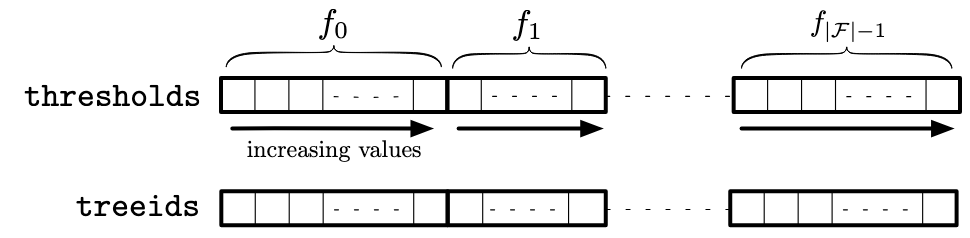
\includegraphics[width=0.8\textwidth]{img/QuickScorer2.png}
    \caption{Data structures used to store the thresholds and the tree IDs.}
\end{figure}
\chapter{Language Models}

Language models are probailistic models of natural language, and are used in many applications such as speech recognition, machine translation, or text generation. In information retrieval, they are used to estimate the probability of a document being relevant to a query by comparing the words contained in both. Language models can be classified in two categories: pure statistical models, and neural models.

\section{Statistical Language Models}
A \textbf{statistical language model} is a probability distribution over sequences of words. Given a sequence of words $w_1 w_2 \dots w_n$, we can compute the probability of the sequence as:
\begin{equation*}
    P(w_1 w_2 \dots w_n) = P(w_1) P(w_2 | w_1) P(w_3 | w_1 w_2) \dots P(w_n | w_1 w_2 \dots w_{n-1})
\end{equation*}
This formula can model any language, but is too impractical to use as it would require to learn the probability of any possible sequence in the language. In practice, language models make assumptions on the probability distribution so that it can be approximated from a relatively limited amount of data; depending on how strong the assumption is, the model will be more or less complex.

A \textbf{unigram model} assumes statistical independence between all words, so that the probability of a sequence is simply calculated as:
\begin{equation*}
    P(d) = P(w_1 w_2 \dots w_n) = P(w_1) P(w_2) \dots P(w_n) = \prod_i^n P(w_i)
\end{equation*}
Sometimes, the logarithm of the probabilities are used instead, transforming the product into a sum:
\begin{equation*}
    \log(\prod_i^n P(w_i)) = \sum_i^n \log(P(w_i))
\end{equation*}
A bayesian classifier that uses this model is also called ``naive'', since it ``naively'' assumes that all words are independent (while, in reality, they are not).

A \textbf{bigram model} assumes statistical dependence of a word from the previous one:
\begin{equation*}
    P(d) = P(w_1 w_2 \dots w_n) = P(w_1) P(w_2 | w_1) P(w_3 | w_2) \dots P(w_n | w_{n-1}) = \prod_i^n P(w_i | w_{i-1})
\end{equation*}
This model is already capable of capturing many language regularities (e.g., verbs followed by nouns or vice-versa, names and expressions formed by multiple words such as ``New York'', ``user friendly'', ``machine learning'', etc.). In general, a \textbf{$\mathbf{n}$-gram model} assumes that the probability of a word depends on the previous $n-1$ words, so the longer the $n$-gram the better the semantic of the language is captured; on the other hand, the model also becomes less statistical significant, as it requires more data to memorize the possible $n$-grams.

\section{Neural Models}
A \textbf{neural model} is a language model that uses neural networks to learn the probability distribution of a language.

\textbf{Word2Vec} is a group of models used to obtain word embeddings, i.e., vector representation of words. These embeddings capture semantic similarity between words, as words that appear in similar contexts will be mapped to similar vectors (in terms of cosine similarity). To capture context, a window of $n$ words is used, where $n$ ranges between 2 and 5 words before and after the central word: longer windows capture more semantic, but less syntax. Even though they solve a prediction task, these models can be trained on any text without any supervision, and are capable of capturing the specific semantic of the source on which they are trained.

Word2Vec can use two architectures: \textbf{CBOW} (\textbf{Continuous Bag Of Words}), or \textbf{skip-gram}. With CBOW, the task is to predict a word given a context (the model is given a sequence, returns a word), while with skip-gram the task is to predict the context given a word (the model is given a word, returns a sequence). Both models are implemented as a two-layer linear neural network where input and output words are represented using one-hot-encoding, and then respectively encoded/decoded into/from a dense representation.

In CBOW, the first layer takes as input the sparse representation of the hot-one-encoded words, produces an abstract representation of the context in the second layer, and finally the output layer converts the abstract representation into a probability vector, where each component represents the probability of a word being in context. The rows produced by the first layer are the embeddings, which are fit during the training process. To test the quality of the embeddings, a test set was developed made of semantic and syntactic relations.

\textbf{FastText} extends Word2Vec by also considering $n$-grams of words. A single word is embedded as the sum of the embeddings of the word itself (as calculated in Word2Vec), and the embeddings of its $n$-grams. For example, the word ``goodbye'' can be represented by the set of its $n$-grams: ``go'', ``goo'', ``ood'', ``odb'', ``dby'', ``bye'', ``ye''. All the $n$-grams are embedded separately, and the same $n$-gram may contribute to the embedding of multiple words. Also, including information about sub-words allows the model to predict the embedding of words it has never seen before (called \textbf{out-of-vocabulary}/\textbf{OOV} words), or to handle misspelled words.

\textbf{Doc2Vec} is an extension of Word2Vec that models the embedding of entire documents. The basic architecture of the model is the same as Word2Vec, but the input is enriched with additional features that identify the document from which the word sequence is from: the output of the first layer is an abstract representation of the words and the identifiers, projected in the same space.

In general, an \textbf{embedding layer} in a neural network is the first layer of the network, and is used to convert the input data into a dense representation specifically designed for the task; it can be initialized with random weights and gradually adjusted during the training phase, or it can be initialized with pre-trained embeddings that are kept fixed (so not modified by the training). Since neural networks process data in batches, and all batches must be of the same length, a \textbf{padding word} is used to fill shorter sequences, adding it before or after its words to reach the desired length.

The latest models are based on deep learning techniques, such as bi-directional character level Long Short Term Memory (LSTM), and multi-headed self-attention (a technique that weighs how important a word is in a sentence based on semantic). These models are cabable of capturing a lot of information about language, but are also very complex and may have up to billions of parameters.

\textbf{Bidirectional Encoder Representation from Transformers} (\textbf{BERT}) is a language model introduced in 2018, designed to pre-train models on large amounts of unlabeled text data which can be fine-tuned to solve specific tasks (e.g., spam detection, topic classification, question answering, text generation). BERT captures the context of a word bidirectionally, considering both words coming before and after the target (unlike other models that only consider the words before). Its architecture is a multi-layer bidirectional Transformer encoder.

The input representation used by BERT can represent both single sentences and pairs of sentences (for example, question-answer pairs). The first token of a sequence is a special \textbf{classification token}, \texttt{[CLS]}. The hidden state corresponding to this token can be then used as a sentence representation for classification tasks. Sentence pairs acked into the same sequence are separated by the special token \texttt{[SEP]}. In addition to the embeddings of the actual words, \textbf{segment embeddings} and \textbf{position embeddings} are used as well. The segment embeddings are used to specify which word belongs to which sentence in the pair (if the input is a pair), while the position embeddings are used to specify the position of the word in the sequence.
\begin{figure}[h]
    \vspace{10pt}
    \centering
    \includesvg[width=0.8\textwidth]{img/bert_input.svg}
    \caption{BERT input representation.}
\end{figure}

BERT is trained on two tasks: Masked Language Model, and Next Sentence Prediction. The \textbf{Masked Language Model} randomly masks some tokens from the input, and the objective is to predict which words are missing based only on the surrounding context. \textbf{Next Sentence Prediction} has the objective of learning wheter two sentences are consecutive or not, providing the model a set of examples of two sentences each, where 50\% of the examples are consecutive and 50\% are not.

\textbf{Self-attention} is a mechanism that computes the importance of a token in a sequence relative to all other tokens; self-attention layers are dedicated layers in the network which produce a set of weights that represent the importance that each token has on every other token in the sequence. \textbf{Multi-headed self-attention} is an extension of self-attention used by BERT that calculates multiple set of weights (in parallel). The output of each ``head'' is concatenated, and passed through a linear layer to combine the information and produce a single output.

\subsection{Neural Approaches for Information Retrieval}

There are two major directions to combining neural models with information retrieval:
\begin{itemize}
    \item \textbf{Interaction-based methods}, where first the term-level similarity between a query and a document is calculated (online) by using their embeddings, and the final ranking is obtained by a neural computation that takes as input the similarities. 
    \item \textbf{Representation-based methods}, where each document and each query is represented separately as a dense vector, obtained through a sequence of neural computations (offline for the documents, online for the queries). The final ranking is based on the similarity of the dense vectors.
\end{itemize}

\paragraph{Interaction-based Methods}
\sloppy
Interaction-based models encode information contained in the query and the document in a single embedding. A model can be trained to produce the ranking score as output. This can be done using BERT, by using the \texttt{[CLS]} token as the aggregated representation of the pair to be used for calculating the score. The model can also be adapted to produce a ranking, either by only considering single query-document pairs, of using a pair-wise approach that considers two documents per query (one relevant, one not relevant).

\fussy
\paragraph{Representation-based Methods}
Representation-based models learn a projection of the (sparse) feature vectors that represent the query and the document into a dense embedding in a low-dimensional space. The models mentioned above all fall in this category. For information retrieval, specifically, the training data is represented by pairs or triples data (so either query-document or query-document1-document2), and the model is trained to produce close embeddings for similar inputs, and distant embeddings for distant inputs. As a loss function, the \textbf{pairwise loss} can be used, which is defined as:
\begin{equation*}
    L(q,d) = \begin{cases}
        d(q,d) & \text{if} \ d \in D^+ \\
        \max(0, m - d(q,d)) &\text{if} \ d \in D^-
    \end{cases}
\end{equation*}
By reducing this loss, the distance between the query and the relevant document is minimized to be as close to 0 as possible, while the distance between the query and the irrelevant document is maximized to be over $m$.

When constructing the dataset, an important aspect is how to choose the negative examples. Positive examples are chosen from supervision, and are always documents that are close to the query. Ideally, the negative examples added to the dataset should be as close as possible to the query (from the \textbf{hard negatives}), so that they are harder to distinguish from positives and the model can learn how to discriminate between them. If the negatives were chosen from documents that are too far (\textbf{easy negatives}), they would be too easy to distinguish and the model would not learn well. Common strategies to selct examples are \textbf{random sampling}, \textbf{in-batch selection} (samples are selected from the same batch as the positive ones), and \textbf{cross-batch selection} (negative samples are selected from different batches).
\begin{figure}[h]
    \centering 
    \includesvg[width=0.5\textwidth]{img/negatives.svg}
    \caption{Negative examples in a dataset. Hard negatives are close to the query, while easy negatives are far.}
\end{figure} \\
Hard negatives can be chosen using two types of sampling: \textbf{static sampling}, in which hard negatives are pre-computed before training and never change, and \textbf{dynamic sampling}, in which hard negatives are chosen as the current top-ranked irrelevant documents produced by the model as it is trained (meaning that the set of hard negatives changes at each step).

To efficiently retrieve documents embedded in dense vectors, the most commonly used algorithm is k-approximate nearest neighbors. Ways to implement the algorithm will be shown in the next chapter. \textbf{Approximate nearest neighbor Negative Contrastive Estimation} (\textbf{ANCE}) is a representation learning method that selects hard negatives dynamically. It uses a BERT Siamese encoder for query and document embeddings, i.e., two identical BERT models that share the same weights but process data individually. Each time a certain number of batches of data is processed, the model stops the training and updates the approximate-nn index used to identify hard negatives.

\textbf{ Contextualized Late Interaction over BERT} (\textbf{ColBERT}) is a model for document ranking that adapts BERT for efficient retrieval. It uses two separate encoders for query and document, producing a term-based representation of them; this means that each document/query is represented by a set of vectors, one per term. This architecture is called \textbf{late interaction}, because document representations can be calculated offline, while query representations are calculated and compared to the documents online. After producing these encodings, the term-wise similarity between them is calculated, and the final similarity is obtained as the sum of the maximum similarities:
\begin{equation*}
    s_{q,d} = \sum_{i \in |E_q|} \max_{j \in |E_d|} E_{q_i} \cdot E_{d_j}^T
\end{equation*}
Here, the similarity is the dot product between the term vectors.
\begin{figure}[h]
    \vspace{15pt}
    \centering
    \includesvg[width=0.70\textwidth]{img/doc_term_sim_colbert.svg}
    \caption{How similarity between query and document is calculated in ColBERT. The term similarities highlighted in red are the ones that are summed to obtain the final similarity.}
\end{figure}

\nocite{*}
\bibliographystyle{unsrt}
\clearpage\bibliography{bibliography}

\end{document}
